\chapter{Geometric Calculus on Manifolds}
\section{Definition of a Vector Manifold}
The definition of a manifold that we will use is - \
\emph{\begin{center}\begin{minipage}{8in}
A vector manifold (generalized surface) is a set of points labeled by vectors lying in a geometric algebra of
arbitrary dimension and signature. If we consider a path in the surface $\f{x}{\lambda}$, the tangent vector is
defined by
\be
x' \equiv \left .\pdiff{\f{x}{\lambda}}{\lambda}\right |_{\lambda_{0}} = \lim_{\epsilon\rightarrow 0}\bfrac{\f{x}{\lambda_{0}+\epsilon}-\f{x}{\lambda_{0}}}{\epsilon}
\ee
and the path length
\be
s \equiv \int_{\lambda_{1}}^{\lambda_{2}} \sqrt{\abs{x'\cdot x'}} d\lambda
\ee
\end{minipage}\end{center}}
\subsection{The Pseudoscalar of the Manifold}
Now introduce a set of paths in the surface all passing through the same point $x$.  These paths define a set of tangent vectors
$\left \{ e_{1},\dots,e_{n}\right \}$.  We assume these paths have been picked so that the vectors are independent and form a basis
for the tangent space at point $x$.  The outer product of the tangent vectors form the pseudoscalar, $\f{I}{x}$, for the tangent space
\be\label{eq346}
	\f{I}{x} \equiv \bfrac{e_{1}\W e_{2}\W\cdots\W e_{n}}{\abs{e_{1}\W e_{2}\W\cdots\W e_{n}}} 
\ee
Thus
\be
	I^{2} = \pm 1
\ee
We require that for any point on the manifold the denominator of equation~\ref{eq346} is nonzero.  We also assume that for all points on the
manifold that $\f{I}{x}$ is continuous, differentiable, singled valued, and has the same grade everywhere.\newline
\subsection{The Projection Operator}\label{sec5_1_2}
Define the projection operator $\Prj{A}$ operating on any multivector $A$ in the embedding multivector space as
\be\label{eq348}
	\Prj{A} \equiv \paren{A\cdot\f{I}{x}}\f{I^{-1}}{x}
\ee
We can show that $\Prj{A}$ extracts those components of $A$ that lie in the geometric algebra defined by $\f{I}{x}$.  Since $\Prj{A}$ is linear
in $A$ if we show that if $\Prj{A_{r}}$ projects correctly for an $r$-grade multivector it will do so for a general mulitvector.  If $n$ is the
dimension of the tangent space and $A_{r}$ is a pure grade multivector we can write equation~\ref{eq348} as
\be
	\Prj{A_{r}} = \left <  A_{r}\f{I}{x}\right >_{\abs{r-n}}\f{I^{-1}}{x}
\ee
Now consider the blades that make up the components of $A_{r}$.  They will either consist only of blades formed from the tangent vectors $e_{i}$ or they will
contain at least one basis vector that is not a tangent vector.  In the first case 
\be
	\left <  A_{r}\f{I}{x}\right >_{\abs{r-n}} = A_{r}\f{I}{x}
\ee
and
\be
	\Prj{A_{r}} = A_{r}
\ee
In the second case there is no component of $A_{r}\f{I}{x}$ of grade $\abs{r-n}$ and
\be
	\Prj{A_{r}} = 0
\ee
This is easily seen if one constructs at point $x$ an orthogonal basis $\paren{o_{i}\cdot o_{j} = \delta_{ij}o^{2}_{i}}$ for the tangent space $\brkt{ o_{1},\dots,o_{n}}$ and an orthogonal basis for
the remainder of the embedding space $\brkt{o_{n+1},\dots,o_{m}}$.  Then any component blade of $A_{r}$ is of the form
\be	
	A_{r}^{i_{1},i_{2},\dots,i_{r}}o_{i_{1}}o_{i_{2}}\dots o_{i_{r}}
\ee
where $i_{1}<i_{2}<\dots <i_{r}$. If $i_{j} \le n \:\forall\: 1 \le j \le r$ then 
\be	
	A_{r}^{i_{1},i_{2},\dots,i_{r}}o_{i_{1}}o_{i_{2}}\dots o_{i_{r}}\cdot I = A_{r}^{i_{1},i_{2},\dots,i_{r}}o_{i_{1}}o_{i_{2}}\dots o_{i_{r}}I
\ee
and
\be	
	\lp A_{r}^{i_{1},i_{2},\dots,i_{r}}o_{i_{1}}o_{i_{2}}\dots o_{i_{r}}\cdot I\rp I^{-1} = A_{r}^{i_{1},i_{2},\dots,i_{r}}o_{i_{1}}o_{i_{2}}\dots o_{i_{r}}
\ee
and 
\be	
	\Prj{A_{r}^{i_{1},i_{2},\dots,i_{r}}o_{i_{1}}o_{i_{2}}\dots o_{i_{r}}} = A_{r}^{i_{1},i_{2},\dots,i_{r}}o_{i_{1}}o_{i_{2}}\dots o_{i_{r}} 
\ee
If any $i_{j} > m$ then $A_{r}^{i_{1},i_{2},\dots,i_{r}}o_{i_{1}}o_{i_{2}}\dots o_{i_{r}}I$ contains no grade $\abs{r-n}$ and
\be
	\Prj{A_{r}^{i_{1},i_{2},\dots,i_{r}}o_{i_{1}}o_{i_{2}}\dots o_{i_{r}}} = 0
\ee
\subsection{The Exclusion Operator}
For an arbitrary multivector $A$ the exclusion operator $\Prjp{A}$ is defined by
\be
	\Prjp{A} \equiv A-\Prj{A}
\ee
\subsection{The Intrinsic Derivative}
Given a set of tangent vectors $\brkt{e_{i}}$ spanning the tangent space and the geometric derivative, $\nabla$, for the embedding space,
the derivative intrinsic to the manifold is defined everywhere by
\be\label{eq5_16}
	\partial \equiv e^{i}e_{i}\cdot\grad = \Prj{\grad}
\ee
Also note that
\be
\Prj{\partial} = \partial
\ee
When we write $\Prj{\grad}$ or $\Prj{\partial}$ the $\grad$ or $\partial$ is not differentiating the $\f{I}{x}$ in the $P$ operator anymore than
$\grad$ is differentiating $dX$ in the fundamental theorem of Geometric Calculus.

We also note that if the vector $a$ is in the tangent space that
\be
	a\cdot\partial = a\cdot\nabla
\ee
and that $a\cdot\partial$ is a scalar operator that gives the directional derivative in the $a$ direction.  Also since it is scalar
it satisfies Leibniz's rules without using the dot notation \color{red}{\bf (remember the convention that if parenthesis are not
present the operator precedence is dot product then wedge product
then geometric product).}\normalcolor
\be
 a\cdot\partial\lp AB \rp = \lp a\cdot\partial A\rp B+ A\lp a\cdot\partial B\rp
\ee
An alternative definition for the intrinsic derivative\footnote{Private conversation with Dr. Alan MacDonald.} is to let $\f{\gamma}{s}$ be a curve
on the manifold.  Then $\deriv{\gamma}{s}$ is a tangent vector to the mainfold and we can define
\be\label{eq5_20}
	\Eval{\deriv{\gamma}{s}}{s=s_{0}}\hspace{-12pt}\cdot\partial \Eval{A}{s=s_{0}} \equiv \Eval{\deriv{\f{A}{\f{\gamma}{s}}}{s}}{s=s_{0}}.
\ee
We can show that equation~\ref{eq5_20} is equivalent to equation~\ref{eq5_16} with the following construction.  Let $\paren{x^{1},\dots,x^{n}}$ be
a local coordinate system for the vector manifold $x=\f{x}{x^{1},\dots,x^{n}}$.  Then a basis for the tangent space is $e_{i}=\pdiff{x}{x^{i}}$ and
the intrinsic derivative is $\partial = e^{i}\pdiff{}{x^{i}}$.  Now write 
\be
	\f{A}{\f{\gamma}{s}} = \f{A}{\f{x^{1}}{s},\dots,\f{x^{n}}{s}}
\ee
so that
\be
	\deriv{\f{A}{\f{\gamma}{s}}}{s} = \pdiff{A}{x^{i}}\deriv{x^{i}}{s}
\ee
but
\be
	\deriv{\gamma}{s} = \pdiff{x}{x^{i}}\deriv{x^{i}}{s} = e_{i}\deriv{x^{i}}{s}
\ee
so that
\be
	\deriv{\gamma}{s}\cdot\partial A = e_{i}\deriv{x^{i}}{s}\cdot e^{j}\pdiff{A}{x^{j}} = \deriv{x^{i}}{s}\pdiff{A}{x^{i}} = \deriv{\f{A}{\f{\gamma}{s}}}{s}
\ee
and the two definitions are equivalent.

\subsection{The Covariant Derivative}
The $\partial$ operator is entirely within the tangent space and if the general multivector function $\f{A}{x}$ is also entirely within the tangent
space, it is still possible (even likely) that $\partial A$ is not entirely within the tangent space.  We need a covariant derivative $D$ that will
result in a multivector entirely within the tangent space.  This can be done by defining
\be
a\cdot D\f{A}{x} \equiv  \Prj{a\cdot\partial\f{A}{x}} 
\ee
so that
\be
 a\cdot\partial A = \Prj{a\cdot\partial A}+\Prjp{a\cdot\partial A} = a\cdot DA + \Prjp{a\cdot\partial A}
\ee
Again since $a\cdot D$ is a scalar operator we have
\be
 a\cdot \f{D}{AB} = \Prj{a\cdot\f{\partial}{AB}} = \lp a\cdot DA\rp B+A\lp a\cdot DB\rp
\ee
A component expansion of $D$ is given in the usual way by (do not forget the summation convention)
\be
 D = e^{i}e_{i}\cdot D
\ee
and
\be
 DA_{r} = e^{i}\lp e_{i}\cdot DA_{r}\rp = \Prj{\partial A_{r}}
\ee
and
\begin{align}
 D\cdot A_{r} \equiv \grade{DA_{r}}{r-1} \\
 D\W A_{r} \equiv \grade{DA_{r}}{r+1}
\end{align}
if $\f{\alpha}{x}$ is a scalar function on the manifold then
\be\label{eq370}
 \partial\f{\alpha}{x} = D\f{\alpha}{x}
\ee
because in equation~\ref{eq370} no basis vectors are differentiated.  To relate $\partial$ and $D$ if the function operated on is 
not a scalar first construct a normalized basis $\set{e_{i}}$ for the tangent space at point $x$.  Then
\be
	I = e_{1}\W e_{2}\W\dots\W e_{n} \mbox{ and } I^{2} = \pm 1
\ee 
and (since $a\cdot\partial$ and $a\cdot D$ are scalar operators we can move them across the wedge products without any problems)
\begin{align}
 \paren{a\cdot\partial I}I^{-1} &= \paren{\sum_{i=1}^{n}e_{1}\W\dots\W\paren{a\cdot De_{i}+\Prjp{a\cdot\partial e_{i}}}\W\dots\W e_{n}}I^{-1} \\
                                &\hspace{-1.5in}= \paren{a\cdot D I}I^{-1}+\sum_{i=1}^{n}\paren{-1}^{i-1}\Prjp{a\cdot\partial e_{i}}\W e_{1}\W\dots\W \breve{e}_{i}\W\dots\W e_{n}I^{-1} \label{eq374}\\
                                &\hspace{-1.5in}= \paren{a\cdot DI}I^{-1}+\Prjp{a\cdot\partial e_{i}}\W e^{i} \label{eq375}
\end{align}
We go from equation~\ref{eq374} to equation~\ref{eq375} by using equation~\ref{eq61} on page~33 in the section on reciprocal frames.

Since $\paren{a\cdot D}I$ is a grade $n$ multivector in the tangent space it must be proportional to $I$ and thus commute with $I$ so that $\paren{\paren{a\cdot\partial} I}I = I\paren{\paren{a\cdot\partial} I}$. Also
$I^{-1} = \pm I$ so that we have
\begin{align}
 \paren{a\cdot DI}I^{-1} &= \pm \paren{a\cdot DI}I \nonumber \\
                                &= \pm\half\paren{\paren{a\cdot DI}I+I\paren{a\cdot DI}} \nonumber \\
                                &= \pm\half\paren{a\cdot D\paren{I^{2}}} \nonumber \\
                                &= 0
\end{align}
Thus
\be\label{eq376}
 \paren{a\cdot\partial I} = \Prjp{a\cdot\partial e_{i}}\W e^{i}I \equiv -\f{S}{a}I
\ee
Where $\f{S}{a}$ is the shape tensor associated with the manifold.  Since $\f{S}{a}$ is a bivector we can write $\paren{A\times B = \paren{AB-BA}/2}$
\be\label{eq377}
 a\cdot\partial I = I\times \f{S}{a}
\ee
since
\be
 \f{S}{a}\cdot I = \f{S}{a}\W I = 0
\ee
and by equation~\ref{eq131} page~58.  Given that $\f{a}{x}$ and $\f{b}{x}$ are vector fields on the manifold (both are in the
tangent space at point $x$), form the expressions in equation~\ref{eq379} (remember that for any three vectors $u$, $v$, and 
$w$ we have $u\cdot\paren{v\W w} = \paren{u\cdot v}w-\paren{u\cdot w}v$)
\begin{align}\label{eq379}
 b\cdot\f{S}{a} &= b\cdot\paren{e^{i}\W\Prjp{a\cdot\partial e_{i}}} \nonumber \\
                &= \paren{b\cdot e^{i}}\Prjp{a\cdot\partial e_{i}}-\paren{b\cdot\Prjp{a\cdot\partial e_{i}}}e^{i} \nonumber \\
                &= \paren{\paren{b^{j}e_{j}}\cdot e^{i}}\Prjp{a\cdot\partial e_{i}} \nonumber \\
                &= b^{j}\delta_{j}^{i}\Prjp{a\cdot\partial e_{i}} \nonumber \\
                &= \Prjp{a\cdot\dot{\partial} b^{i}\dot{e}_{i}}
\end{align}
but
\begin{align}
 \Prjp{a\cdot\partial b} &= \Prjp{a\cdot\partial\paren{b^{i}e_{i}}} \nonumber \\
                         &= \Prjp{a\cdot\dot{\partial}\dot{b}^{i}e_{i}+a\cdot\dot{\partial}b^{i}\dot{e}_{i}} \nonumber \\
                         &= \Prjp{a\cdot\dot{\partial}b^{i}\dot{e}_{i}} 
\end{align}
and
\color{red}
\be
\fbox{$b\cdot\f{S}{a} = \Prjp{a\cdot\partial b}$}
\ee
\normalcolor
Thus
\be
 a\cdot\partial b = \Prj{a\cdot\partial b}+\Prjp{a\cdot\partial b} = a\cdot Db+b\cdot\f{S}{a}
\ee
and (using the fact that the dot product of a vector and bivector are antisymmetric)
\be
 a\cdot Db = a\cdot\partial b + \f{S}{a}\cdot b
\ee
Now consider the expression
\begin{align}
 a\cdot \f{D}{b_{1}\dots b_{r}} &= \sum_{i=1}^{r}b_{1}\dots\paren{a\cdot\partial b_{i}+\f{S}{a}\cdot b_{i}}\dots b_{r} \nonumber \\
                                &= \sum_{i=1}^{r}b_{1}\dots\paren{a\cdot\partial b_{i}}\dots b_{r}+ \nonumber \\
                                &\hspace{1in}\sum_{i=1}^{r}b_{1}\dots\paren{\f{S}{a}\cdot b_{i}}\dots b_{r} \nonumber \\
                                &= a\cdot\f{\partial}{b_{1}\dots b_{r}}+ \nonumber \\
                                &\hspace{1in}\half\sum_{i=1}^{r}b_{1}\dots\paren{\f{S}{a}b_{i}-b_{i}\f{S}{a}}\dots b_{r} \nonumber \\
                                &= a\cdot\f{\partial}{b_{1}\dots b_{r}}+\half\paren{\f{S}{a}\paren{b_{1}\dots b_{r}}-\paren{b_{1}\dots b_{r}}\f{S}{a}}+\nonumber \\
                                &\hspace{1in}\half\paren{\sum_{i=2}^{r-1}b_{1}\dots\f{S}{a}b_{i}\dots b_{r}-\sum_{i=2}^{r-1}b_{1}\dots b_{i}\f{S}{a}\dots b_{r}} +\nonumber \\
                                &\hspace{1in}\half\paren{b_{1}\dots b_{r-1}\f{S}{a}b_{r}-b_{1}\f{S}{a}b_{2}\dots b_{r}}\nonumber \\
                                &= a\cdot\f{\partial}{b_{1}\dots b_{r}}+\half\paren{\f{S}{a}\paren{b_{1}\dots b_{r}}-\paren{b_{1}\dots b_{r}}\f{S}{a}}+\nonumber \\
                                &\hspace{1in}\half\paren{\sum_{i=3}^{r-1}b_{1}\dots\f{S}{a}b_{i}\dots b_{r}-\sum_{i=2}^{r-2}b_{1}\dots b_{i}\f{S}{a}\dots b_{r}} +\label{eq384} \\                               
                                &= a\cdot\f{\partial}{b_{1}\dots b_{r}}+\f{S}{a}\times\paren{b_{1}\dots b_{r}} \label{eq385}
\end{align}
To get from equation~\ref{eq384} to equation~\ref{eq385} note that in the sums in parenthesis in equation~\ref{eq384} the $i^{th}$ term in the first sum cancels the
$i^{th}+1$ term in the second sum.

Since any multivector is a linear superposition of terms containing $b_{1}\dots b_{r}$ with $1 \le r \le n$ and a scalar we have
\color{red}
\be\label{eq386}
\fbox{$a\cdot DA = a\cdot\partial A + \f{S}{a}\times A $}
\ee
\normalcolor
Where $\f{a}{x}$ and $\f{b}{x}$ are vector fields on the manifold write
\be\label{eq387}
 a\cdot\partial b = a\cdot\partial\Prj{b} = a\cdot\dot{\partial}\f{\dot{\prj}}{b}+\Prj{a\cdot\partial b} = a\cdot\dot{\partial}\f{\dot{\prj}}{b}+a\cdot Db
\ee
Now substitute equation~\ref{eq386} into equation~\ref{eq387} to get
\be\label{eq5_45}
 a\cdot\dot{\partial}\f{\dot{\prj}}{b} = b\cdot\f{S}{a}
\ee
\section{Coordinates and Derivatives}
In a region of the manifold we introduce local coordinates $x^{i}$ and define the frame vectors as
\be
 e_{i} = \pdiff{x}{x^{i}}
\ee
From the definition of $\partial$ is follows that $e^{i} = \partial x^{i}$.  The $\brkt{e_{i}}$ are referred to
as tangent vectors and the reciprocal frame $\brkt{e^{i}}$ as the cotangent vector (or 1-forms). The covariant
derivative along a coordinate vector, $e_{i}\cdot D$, satisfies and defines both $D_{i}$ and $S_{i}$.
\color{red}
\be
 \fbox{$e_{i}\cdot DA = D_{i}A = e_{i}\partial A+\f{S}{e_{i}}\times A \equiv \partial_{i}A+S_{i}\times A$}
\ee
\normalcolor
The tangent frame vectors satisfy
\be\label{eq422}
 \partial_{i}e_{j}-\partial_{j}e_{i} = \paren{\partial_{i}\partial_{j}-\partial_{j}\partial_{i}}x = 0
\ee
Using the $\prj$ operator on equation~\ref{eq422} gives
\be\label{eq426}
 D_{i}e_{j} - D_{j}e_{i} = 0
\ee
while using $\prj_{\perp}$ gives
\be\label{eq424}
 e_{i}\cdot S_{j} = e_{j}\cdot S_{i}
\ee
For arbitrary vectors $a$ and $b$ in the tangent space equation~\ref{eq424} becomes
\be\label{eq5_51}
 a\cdot\f{S}{b} = b\cdot\f{S}{a} 
\ee
In terms of the coordinate vectors the shape tensor becomes
\color{red}
\be
 \fbox{$\f{S}{a} = e^{k}\W\Prjp{a\cdot\partial e_{k}}$}
\ee
\normalcolor
and
\be
 S_{i} = e^{k}\W\Prjp{e_{i}\cdot\partial e_{k}} = e^{k}\W\Prjp{e_{k}\cdot\partial e_{i}}
\ee
Then
\be
 \partial\W e_{i} = e^{k}\W\partial_{k}e_{i} = e^{k}\W\paren{\Prj{\partial_{k}e_{i}}+\Prjp{\partial_{k}e_{i}}} = D\W e_{i}+S_{i}
\ee
Letting $a = a^{i}e_{i}$ be a constant vector in the tangent space gives the general result
\color{red}
\be
 \fbox{$\partial\W a = D\W a+\f{S}{a}$}
\ee
\normalcolor
Additionally
\begin{align}
  \partial\W a &= \partial\W\paren{\Prj{a}} \nonumber \\
               &= \dot{\partial}\W\f{\dot{\prj}}{a}+\Prj{\partial\W a} \nonumber \\
               &= D\W a + \dot{\partial}\W\f{\dot{\prj}}{a}
\end{align}
Thus
\be
 \dot{\partial}\W\f{\dot{\prj}}{a} = \f{S}{a}
\ee
Note that if $a$ and $b$ are any two vectors in the embedding space then $\Prj{a\W b}=\Prj{a}\W\Prj{b}$ and if $\f{\phi}{x}$ is a scalar function on the
manifold we have
\begin{align}
 \partial\W\partial\phi &= \partial\W\Prj{\nabla\phi} \nonumber \\
                        &= \dot{\partial}\W\Prj{\dot{\nabla\phi}} + \dot{\partial}\W\f{\dot{\prj}}{\nabla\phi} \nonumber \\
                        &= \Prj{\dot{\nabla}}\W\Prj{\dot{\nabla\phi}} + \dot{\partial}\W\f{\dot{\prj}}{\nabla\phi} \nonumber \\
                        &= \Prj{\nabla\W\nabla\phi}+ \dot{\partial}\W\f{\dot{\prj}}{\nabla\phi}
\end{align}
but $\nabla\W\nabla = 0$ so
\be
 \partial\W\partial\phi = \f{S}{\nabla\phi}
\ee
Since $\f{S}{a}$ for any vector $a$ lies outside the manifold we have
\be
 D\W\paren{D\phi} = 0
\ee
Letting $\f{\phi}{x} = \f{x^{i}}{x}$, then since $\f{x^{i}}{x}$ is a scalar function
\be\label{eq438a}
D\W\paren{Dx^{i}} = D\W e^{i} = 0
\ee
so that for a general vector $a = \f{a_{i}}{x}e^{i}$ we have
\be\label{eq436}
 D\W a = D\W\paren{a_{j}e^{j}} = e^{i}\W e^{j}\paren{\partial_{i}a_{j}} = \half e^{i}\W e^{j}\paren{\partial_{i}a_{j}-\partial_{j}a_{i}}
\ee
Equation~\ref{eq436} is isomorphic to the definition of the {\em exterior derivative} of differential geometry.
\section{Riemannian Geometry}
We shall now relate the shape tensor to the metric tensor and Christoffel connection.  The metric tensor is defined by
\be
 g_{ij} \equiv e_{i}\cdot e_{j}
\ee
and the Christoffel connection by
\be
 \Gamma^{i}_{jk} \equiv \paren{D_{j}e_{k}}\cdot e^{i}
\ee
so that the components of the covariant derivative are given by
\begin{align}
 \paren{a\cdot Db}\cdot e^{i} &= a^{j}\paren{D_{j}\paren{b^{k}e_{k}}}\cdot e^{i} \nonumber \\
                              &= a^{j}\paren{\partial_{j}b^{i}+\Gamma^{i}_{jk}b^{k}}
\end{align}
The $\Gamma^{i}_{jk}$ can be expressed in terms of the $g_{ij}$ by considering the following relations. First,
the $\Gamma^{i}_{jk}$ are symmetric in the $j$ and $k$ indices.
\be\label{eq440}
 \Gamma^{i}_{jk} - \Gamma^{i}_{kj} = \paren{D_{j}e_{k}-D_{k}e_{j}}\cdot e^{i} = 0
\ee
Second, the curl of the basis vectors is given by (equation~\ref{eq438a})
\be\label{eq441}
 D\W e_{i} = D\W\paren{g_{ij}e^{j}} = \paren{Dg_{ij}}\W e^{j}
\ee
By equation~\ref{eq440} we can write
\begin{align}
 \Gamma^{i}_{jk} &= \half e^{i}\cdot\paren{D_{j}e_{k}+D_{k}e_{j}} \nonumber \\
                 &= \half e^{i}\cdot\paren{\paren{e_{j}\cdot D}e_{k}+\paren{e_{k}\cdot D}e_{j}} \label{eq442}
\end{align}
Now apply equation~\ref{eq450} (Appendix A) and equation~\ref{eq441} to each term in equation~\ref{eq442} to get
\begin{align}
 \paren{e_{j}\cdot D}e_{k} + \paren{e_{k}\cdot D}e_{j} &= e_{j}\cdot\paren{D\W e_{k}}+e_{k}\cdot\paren{D\W e_{j}} + 
                                                          \paren{e_{j}\cdot\dot{e}_{k}}\dot{D}+\paren{e_{k}\cdot\dot{e}_{j}}\dot{D} \nonumber \\
                                                       &= e_{j}\cdot\paren{D\W e_{k}}+e_{k}\cdot\paren{D\W e_{j}} + D\paren{g_{jk}}\nonumber \\
                                                       &= e_{j}\cdot\paren{\paren{Dg_{kl}}\W e^{l}}+e_{k}\cdot\paren{\paren{Dg_{jl}}\W e^{j}} + D\paren{g_{jk}}
\end{align}
Now apply equation~\ref{eq447} (Appendix A) to $e_{j}\cdot\paren{Dg_{kl}\W e^{l}}$ and $e_{k}\cdot\paren{Dg_{jl}\W e^{j}}$ giving in the first case
\begin{align}
  e_{j}\cdot\paren{Dg_{kl}\W e^{l}} &= \paren{e_{j}\cdot\paren{Dg_{kl}}}e^{l}-\paren{e_{j}\cdot e^{l}}Dg_{kl} \nonumber \\
                                    &= \paren{\paren{e_{j}\cdot D}g_{kl}}e^{l}-\delta_{j}^{l}Dg_{kl} \nonumber \\
                                    &= \paren{D_{j}g_{kl}}e^{l}-Dg_{kj} \nonumber \\
                                    &= \paren{\partial_{j}g_{kl}}e^{l}-\partial g_{kj}
\end{align}
so that equation~\ref{eq442} becomes
\begin{align}
 \Gamma^{i}_{jk} &= \half e^{i}\cdot \paren{\paren{\partial_{j}g_{kl}}e^{l}+\paren{\partial_{k}g_{jl}}e^{l}-\partial g_{kj}} \nonumber \\
                 &= \half e^{i}\cdot \paren{\paren{\partial_{j}g_{kl}}e^{l}+\paren{\partial_{k}g_{jl}}e^{l}-e^{l}\partial_{l} g_{kj}} \nonumber \\
                 &= \half g^{il} \paren{\partial_{j}g_{kl}+\partial_{k}g_{jl}-\partial_{l} g_{kj}}
\end{align}
which is the standard formula for the $\Gamma^{i}_{jk}$. 

Now define the commutator bracket $\cbrk{A}{B}$ of the multivectors $A$ and $B$ by (note there is no $\half$ factor)
\be
 \cbrk{A}{B} \equiv AB-BA
\ee
Now form equation~\ref{eq447} (Appendix A) and use the Jacobi identity (equation~\ref{jacobi}) to reduce the double commutator products on the r.h.s. of the equation
\begin{align}
\cbrk{D_{i}}{D_{j}}A &= \partial_{i}\paren{\partial_{j}A+S_{j}\times A}+S_{i}\times\paren{\partial_{j}A+S_{j}\times A}
                      -\partial_{j}\paren{\partial_{i}A+S_{i}\times A}-S_{j}\times\paren{\partial_{i}A+S_{i}\times A} \nonumber \\
                     &= \paren{\partial_{i}S_{j}-\partial_{j}S_{i}}\times A +\paren{S_{i}\times S_{j}}\times A \label{eq448}
\end{align}
However (see equations~\ref{eq376} and \ref{eq377}, page 153) so that $S_{i} = -\paren{\partial_{i}I}I^{-1}$, and
\begin{align}
 \paren{\partial_{i}S_{j}-\partial_{j}S_{i}} &= -\partial_{i}\paren{\paren{\partial_{j}I}I^{-1}}+\partial_{j}\paren{\paren{\partial_{i}I}I^{-1}} \nonumber \\
                                             &= \paren{\partial_{j}I}\paren{\partial_{i}I}I^{-2}-\paren{\partial_{i}I}\paren{\partial_{j}I}I^{-2} \nonumber \\
                                             &= \paren{\partial_{j}I}I^{-1}\paren{\partial_{i}I}I^{-1}-\paren{\partial_{i}I}I^{-1}\paren{\partial_{j}I}I^{-1} \nonumber \\
                                             &= S_{j}S_{i}-S_{i}S_{j} = -2S_{i}\times S_{j} \label{eq448a}
\end{align}
where we have used that $I^{-1}$ and the partial derivatives of $I$ commute to reduce the second line of equation~\ref{eq448a}
\be\label{eq8_30}
\cbrk{D_{i}}{D_{j}}A = -\paren{S_{i}\times S_{j}}\times A
\ee
The commutator of the covariant derivatives defines the Riemann tensor
\be\label{eq451}
 \Rten{a,b} \equiv \Prj{\f{S}{b}\times\f{S}{b}}
\ee
Since $\Rten{a,b}$ is a bilinear antisymmetric function of $a$ and $b$ we may write
\be\label{eq452}
 \Rten{a\W b} = \Prj{\f{S}{b}\times\f{S}{a}}
\ee
or
\be
 \Rten{e_{i}\W e_{j}} = \Prj{\f{S}{e_{j}}\times\f{S}{e_{i}}}
\ee
Since both $\f{S}{a}$ and $\f{S}{b}$ are bivectors we can use equation~\ref{eq453} (Appendix A) to reduce $\f{S}{b}\times\f{S}{a}$
\begin{align}
\f{S}{b}\times\f{S}{a} &= \paren{e^{k}\W\Prjp{b\cdot\partial e_{k}}}\times\paren{e^{l}\W\Prjp{a\cdot\partial e_{l}}} \nonumber \\
                       &= \paren{e^{k}\cdot\Prjp{a\cdot\partial e_{l}}}\Prjp{b\cdot\partial e_{k}}\W e^{l}
                       -\paren{e^{k}\cdot e^{l}}\Prjp{b\cdot\partial e_{k}}\W\Prjp{a\cdot\partial e_{l}} \nonumber \\
                       & +\paren{\Prjp{b\cdot\partial e_{k}}\cdot e^{l}}e^{k}\W\Prjp{a\cdot\partial e_{l}} 
                       -\paren{\Prjp{b\cdot\partial e_{k}}\cdot \Prjp{a\cdot\partial e_{l}}}e^{k}\w e^{l} \label{eq452}
\end{align}
In equation~\ref{eq452} the first and third terms are zero. The second term is entirely outside the tangent space  and the fourth term
is entirely inside the tangent space.  Also note that since the second term consists of bivectors that are entirely outside the tangent 
space that term commutes with all multivectors $A$ in the tangent space so that the commutator of the second term with $A$ is zero. Thus
the Riemann tensor reduces to
\be\label{eq454}
\Rten{a\W b} = -\paren{\Prjp{b\cdot\partial e_{u}}\cdot \Prjp{a\cdot\partial e_{v}}}e^{u}\w e^{v}
\ee 
or
\be\label{eq455}
\Rten{e_{i}\W e_{j}} = -\paren{\Prjp{\partial_{j} e_{u}}\cdot \Prjp{\partial_{i} e_{v}}}e^{u}\w e^{v}
\ee
To calculate the Riemann tensor in terms of the Christoffel symbols note that
\begin{align}
	\cbrk{D_{i}}{D_{j}}e_{k} &= \paren{S_{j}\times S_{i}}\times e_{k}  \label{eq5_82} \\
	                         &= \paren{S_{j}\times S_{i}}\cdot e_{k}  \label{eq5_83} \\
	                         &= \Rten{e_{i}\W e_{j}}\cdot e_{k} \label{eq5_84}
\end{align}
Equation~\ref{eq5_82} comes from letting $A = e_{k}$ in equation~\ref{eq8_30}. Equation~\ref{eq5_83} comes from
the fact that $S_{j}\times S_{i}$ is a bivector and that the commutator product of a bivector and a vector is the
same as the dot product.  Finally we have that $\paren{S_{j}\times S_{i}}\cdot e_{k} = \Prj{S_{j}\times S_{i}}\cdot e_{k}$ 
since from equation~\ref{eq452} $\Prjp{S_{j}\times S_{i}} = -\paren{e^{m}\cdot e^{l}}\Prjp{e_{j}\cdot\partial e_{m}}\W\Prjp{e_{i}\cdot\partial e_{l}}$
so that $\Prjp{S_{j}\times S_{i}}\cdot e_{k} = 0$. Thus
\begin{align}
\Rten{e_{i}\W e_{j}}\cdot e_{k} &= \cbrk{D_{i}}{D_{j}}e_{k} \nonumber \\
                                &= D_{i}\paren{\Gamma_{jk}^{a}e_{a}}-D_{j}\paren{\Gamma_{ik}^{a}e_{a}} \nonumber \\
                                &= \paren{\partial_{i}\Gamma_{jk}^{a}}e_{a}+\Gamma_{jk}^{a}D_{i}e_{a}
                                 -\paren{\partial_{j}\Gamma_{ik}^{a}}e_{a}-\Gamma_{ik}^{a}D_{j}e_{a} \nonumber \\
                                &= \paren{\partial_{i}\Gamma_{jk}^{a}+\Gamma_{jk}^{b}\Gamma_{ib}^{a}}e_{a} 
                                 -\paren{\partial_{j}\Gamma_{ik}^{a}-\Gamma_{ik}^{b}\Gamma_{jb}^{a}}e_{a} 
\end{align}
so
\begin{align}
\paren{\Rten{e_{i}\W e_{j}}\cdot e_{k}}\cdot e^{l} &= \paren{\paren{\partial_{i}\Gamma_{jk}^{a}}+\Gamma_{jk}^{b}\Gamma_{ib}^{a}}\delta_{a}^{l}
                                                   -\paren{\paren{\partial_{j}\Gamma_{ik}^{a}}+\Gamma_{ik}^{b}\Gamma_{jb}^{a}}\delta_{a}^{l} \nonumber \\
                                                   &= \partial_{i}\Gamma_{jk}^{l}+\Gamma_{jk}^{b}\Gamma_{ib}^{l}
                                                   -\partial_{j}\Gamma_{ik}^{l}-\Gamma_{ik}^{b}\Gamma_{jb}^{l}
\end{align}
Using equation~\ref{eq455} we have
\be\label{eq458}
\paren{\Rten{e_{i}\W e_{j}}\cdot e_{k}}\cdot e^{l} = -\paren{\Prjp{\partial_{j} e_{u}}\cdot \Prjp{\partial_{i} e_{v}}}\paren{\paren{e^{u}\w e^{v}}\cdot e_{k}}\cdot e^{l} 
\ee
Using equation~\ref{eq465} (Appendix A) to reduce $\paren{\paren{e^{u}\w e^{v}}\cdot e_{k}}\cdot e^{l}$ gives
\be\label{eq459}
\paren{\paren{e^{u}\w e^{v}}\cdot e_{k}}\cdot e^{l} = g^{ul}\delta_{k}^{v}-g^{vl}\delta_{k}^{u}
\ee
Substituting equation~\ref{eq459} into equation~\ref{eq458} gives
\begin{align}
\paren{\Rten{e_{i}\W e_{j}}\cdot e_{k}}\cdot e^{l} &= \Prjp{\partial_{j} e_{k}}\cdot \Prjp{\partial_{i} e_{v}}g^{vl}
                                                    -\Prjp{\partial_{j} e_{u}}\cdot \Prjp{\partial_{i} e_{k}}g^{ul} \nonumber \\
                                                   &= \Prjp{\partial_{j} e_{k}}\cdot \Prjp{\partial_{i} e^{l}}
                                                    -\Prjp{\partial_{j} e^{l}}\cdot \Prjp{\partial_{i} e_{k}}
\end{align}
because
\begin{align}
\Prjp{\partial_{i} e_{v}}g^{vl} &= \Prjp{g^{vl}\partial_{i} e_{v}} \nonumber \\
                                &= \Prjp{\partial_{i}\paren{g^{vl}e_{v}}-\paren{\partial_{i}g^{vl}}e_{v}} \nonumber \\
                                &= \Prjp{\partial_{i}\paren{g^{vl}e_{v}}} \nonumber \\
                                &= \Prjp{\partial_{i}e^{l}}
\end{align}
Finally
\begin{align}
R\indices{_{ijk}^{l}} &= \Prjp{\partial_{j} e_{k}}\cdot \Prjp{\partial_{i} e^{l}}-\Prjp{\partial_{j} e^{l}}\cdot \Prjp{\partial_{i} e_{k}} \nonumber \\
                &= \partial_{i}\Gamma_{jk}^{l}+\Gamma_{jk}^{b}\Gamma_{ib}^{l}-\partial_{j}\Gamma_{ik}^{l}-\Gamma_{ik}^{b}\Gamma_{jb}^{l}       
\end{align}
Which is the standard form of the Riemann tensor in terms of the Christoffel symbols. Note that
\begin{align}
 R_{ijkl} &= R\indices{_{ijk}^{v}}g_{vl} \nonumber \\
          &= \Prjp{\partial_{j} e_{k}}\cdot \Prjp{\partial_{i} e_{l}}-\Prjp{\partial_{j} e_{l}}\cdot \Prjp{\partial_{i} e_{k}} \label{eq466}
\end{align}
From equation~\ref{eq466} and equation~\ref{eq422} $\paren{\partial_{i}e_{j}=\partial_{j}e_{i}}$ we can see that the symmetries of the covariant Riemann tensor are
\be 
R_{ijkl} = -R_{jikl},\:\: R_{ijkl} = -R_{ijlk},\mbox{ and } R_{ijkl} = R_{klij}\nonumber
\ee
To prove the first Bianchi identity form $\Rten{e_{i}\W e_{j}}\cdot e_{k}$ and use equation~\ref{eq426} $\paren{D_{j}e_{k}=D_{k}e_{j}}$ to get
\begin{align}
\Rten{e_{i}\W e_{j}}\cdot e_{k} &= D_{i}D_{j}e_{k}-D_{j}D_{i}e_{k} \nonumber \\
                                &= D_{i}D_{k}e_{j}-D_{j}D_{k}e_{i} \nonumber \\
                                &= \cbrk{D_{i}}{D_{k}}e_{j}-\cbrk{D_{j}}{D_{k}}e_{i}+D_{k}\paren{D_{i}e_{j}-D_{j}e_{i}} \nonumber \\
                                &= \Rten{e_{i}\W e_{k}}\cdot e_{j}-\Rten{e_{j}\W e_{k}}\cdot e_{i}
\end{align}
now defining the function $\f{F}{a,b,c}$ by
\be\label{eq468}
\f{F}{a,b,c} \equiv a\cdot\Rten{b\W c}+c\cdot\Rten{a\W b}+b\cdot\Rten{c\W a} = 0
\ee
However $\f{F}{a,b,c}$ is a linear function of $a$, $b$, and $c$.  Also $\f{F}{b,a,c} = -\f{F}{a,b,c}$ and
$\f{F}{a,c,b} = -\f{F}{a,b,c}$ so since $F$ is antisymmetric in all arguments we may write
\be\label{eq469}
\f{F}{a,b,c} = \f{F}{a\W b\W c}
\ee 
Thus equation~\ref{eq468} contains $n\binom{n}{3} = \bfrac{n^{2}\paren{n-1}\paren{n-2}}{6}$ scalar coefficients. Since the
Riemann tensor is a bivector valued function of a bivector the degrees of freedom of the tensor is no more than
$\paren{\bfrac{n\paren{n-1}}{2}}^{2}$ and equation~\ref{eq468} reduces the degrees of freedom by $n\binom{n}{3}$ so that
the total degrees of freedom of the Riemann tensor is
\be\nonumber
\paren{\bfrac{n\paren{n-1}}{2}}^{2}-n\binom{n}{3} = \bfrac{1}{12}n^{2}\paren{n^{2}-1}.
\ee

\section{Manifold Mappings}
One way of illuminating the connection between geometric calculus on manifolds and the standard presentation of differential geometry
is to study the effects of mappings from one manifold to another (including mapping of the manifold onto itself). Let 
$f:\mathcal{M}\rightarrow\mathcal{M}'$ define a mapping from the manifold $\mathcal{M}$ to $\mathcal{M}'$.  For our purposes $f$ is a
diffeomorphism.  That is $f$ and all of its derivatives are continuous and invertible. Thus we can show that the tangent spaces of 
$\mathcal{M}$ and $\mathcal{M'}$ are of the same dimension.  We shall denote the image of $x \in \mathcal{M}$
as $x'$ so that $\f{f}{x} = x'$. Then if $\f{x}{\lambda}$ defines a curve on $\mathcal{M}$, then $\f{f}{\f{x}{\lambda}} = \f{x'}{\lambda}$
defines a curve on $\mathcal{M'}$.  In summary -
\begin{center}
\begin{tabular}{cl}
$\mathcal{M}$: & Manifold embedded in vector space $V$ ($\mathcal{M} \subset V$) \\
$s^{i}$: & Coordinates of manifold $\mathcal{M}$ such that $\f{x}{s^{1},\dots,s^{r}} \in \mathcal{M}\subset V$, $\f{\dim}{V} > r$ \\
$u_{i}$: & Basis vectors for embedding space $V$ ($x=x^{i}u_{i}\in\mathcal{M}$)\\
$\f{x}{\lambda}$: & Trajectory in $\mathcal{M}$ such that $\f{x}{\lambda} = \f{x}{\f{s^{1}}{\lambda},\dots,\f{s^{r}}{\lambda}}$ \\
$\mathcal{M'}$: & Manifold embedded in vector space $V'$ \\
$u'_{i}$: & Basis vectors for $V'$  \\
$f$: & Diffeomorphism from $V$ to $V'$ \\
$x'$: & Element of $\mathcal{M'}$ as an image of $x\in\mathcal{M}$ ($x'=\f{f}{x}\in\mathcal{M'}\subset V'$) \\
$f^{i}$: & Component of $f$ in $V'$ such that $\f{f}{x}=\f{f^{i}}{x}u'_{i}$
\end{tabular}
\end{center}
Since $\deriv{x}{\lambda}$ is in the tangent space of $\mathcal{M}$ and (remember that the dot product comes 
before the geometric product)
\begin{align}
	\deriv{x'}{\lambda} &= \deriv{}{\lambda}\paren{\f{f}{\f{x}{\lambda}}} \nonumber \\
	&= \paren{\deriv{x}{\lambda}\cdot\partial}\f{f}{x} \nonumber \\
	&=\paren{\deriv{s^{i}}{\lambda}\pdiff{x}{s^{i}}\cdot e^{k}\partial_{k}}\paren{\f{f^{j}}{x}u'_{j}} \nonumber \\
	&=\paren{\deriv{s^{i}}{\lambda}e_{i}\cdot e^{k}\partial_{k}}\paren{\f{f^{j}}{x}u'_{j}}  \nonumber \\
	&=\paren{\deriv{s^{i}}{\lambda}\delta_{i}^{k}\partial_{k}}\paren{\f{f^{j}}{x}u'_{j}}  \nonumber \\
	&=\deriv{s^{i}}{\lambda}\pdiff{f^{j}}{s^{i}}u'_{j}
\end{align}
is in the tangent space of $\mathcal{M}'$.  Thus if $a$ is in
the tangent space of $\mathcal{M}$ at point $x$ then
\be\label{eq5_94}
 a' = \paren{a\cdot\partial}\f{f}{x} = \f{\sff}{a;x} = \f{\sff}{a}
\ee
is in the tangent space of $\mathcal{M}'$ at point $x'$ and the frame (basis) vectors for $\mathcal{M}$ at point $x$ map from one tangent
space to the other via
\be\label{eq5_95}
 e'_{i} = \paren{e_{i}\cdot\partial}\f{f}{x} = \f{\sff}{e_{i};x} = \f{\sff}{e_{i}}
\ee
where in the rhs of equations~\ref{eq5_94} and \ref{eq5_95} we suppress the position dependence, $x$, in the linear functional $\sff$. Since
$\f{f}{x}$ is invertible for all derivatives there is no $e_{i}$ such that $\f{\sff}{e_{i}}=0$ (the dimension of the image tangent space is
the same as the original).  Note that we actually have $\f{e_{i}}{x}$ and  $\f{e'_{i}}{x}$. An example is shown in figure~\ref{mercator}

\begin{figure}[tbp]
\begin{center}
\vspace{-0.5in}
\scalebox{0.8}{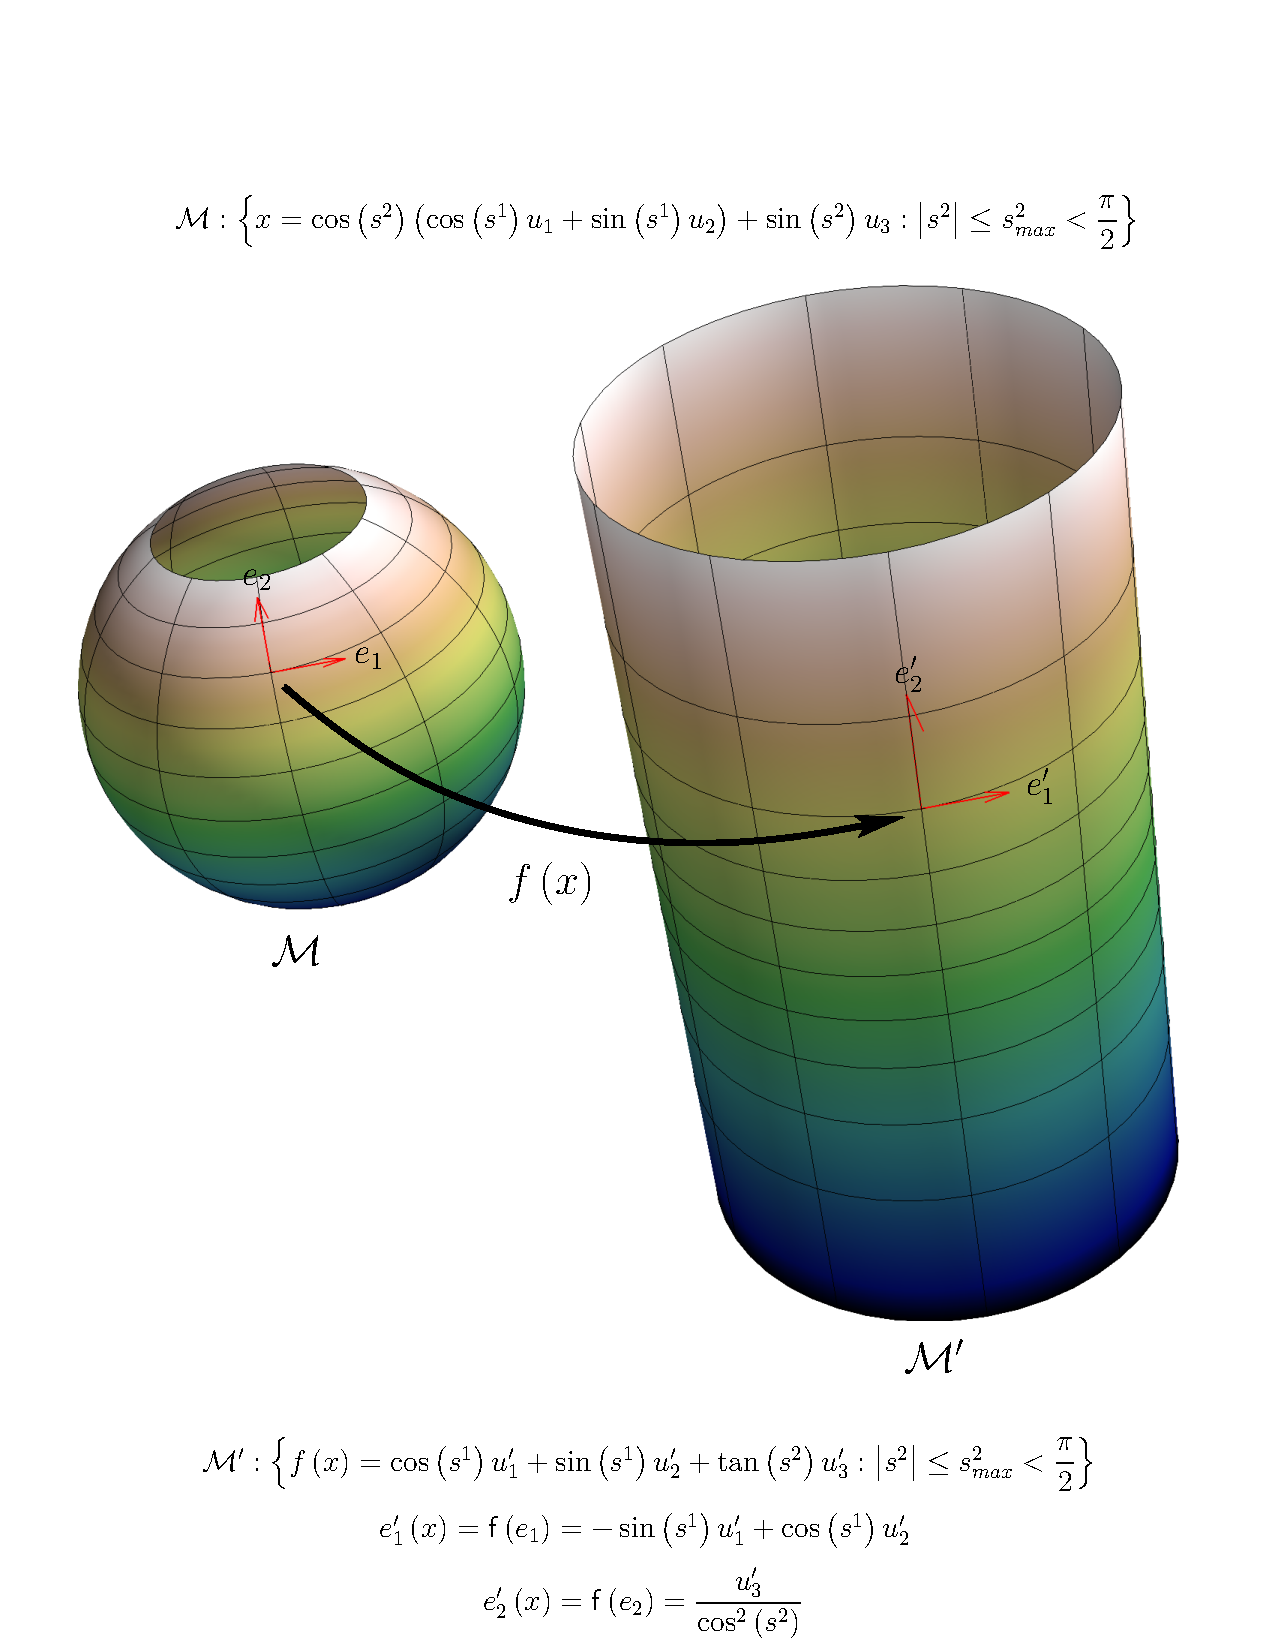
\includegraphics{mercator_annotated.pdf}}
\caption{Mercator mapping of sphere to cylinder manifold. Top and bottom of sphere excluded.}\label{mercator}
\end{center}
\end{figure} 

The cotangent frame, $e^{i}$, in $\mathcal{M}$ is mapped to $e'^{i}$ in $\mathcal{M}'$
via the adjoint of the inverse
\be
e'^{i} = \f{\overline{\sff^{-1}}}{e^{i}}.
\ee
This is simply proved by noting (remember that by definition $a\cdot\f{\bar{\sff}}{b} = b\cdot\f{\sff}{a}$)
\begin{align}
	e'_{i}\cdot e'^{j} &= \f{\sff}{e_{i}}\cdot\f{\overline{\sff^{-1}}}{e^{j}} \nonumber \\
	                   &= e^{j}\cdot\f{\sff^{-1}}{\f{\sff}{e_{i}}} \nonumber \\
                       &= e^{j}\cdot e_{i} \nonumber \\
                       &= \delta_{i}^{j}
\end{align}
The exterior product of two tangent vectors, $e_{i}\W e_{j}$, maps to
\be
	e_{i}\W e_{j} \mapsto  e'_{i}\W e'_{j} = \f{\sff}{e_{i}\W e_{j}}
\ee
since $\sff$ is linear in tangent space arguments.  Likewise if $I'$ is the ``unit" pseudoscalar for the tangent 
space of $\mathcal{M'}$ at $\f{f}{x}$ 
($I'^{2}=\pm 1$) and $I$ the ``unit" pseudoscalar for the tangent space of $\mathcal{M}$ at $x$ ($I^{2}=\pm 1$) then
\be\label{5_102}
	 \f{\sff}{I} = \f{\det}{\sff}I'.
\ee
Since $\sff$ is invertible (the tangent space and its image are isomorphic) we can apply the definition of determinant in 
equation~\ref{1_79} to equation~\ref{5_102}.  For cotangent vectors $e^{i}$ and $e^{j}$
\be
	e'^{i}\W e'^{j} \mapsto \f{\overline{\sff^{-1}}}{e^{i}}\W\f{\overline{\sff^{-1}}}{e^{j}} = \f{\overline{\sff^{-1}}}{e^{i}\W e^{j}}. 
\ee
Since the derivative of a scalar field, $\phi$, is a cotangent vector $\partial\phi = e^{i}\partial_{i}\phi$ and 
$\f{\phi}{x} = \f{\phi'}{x'}$ we can write
\be
	\partial' = \f{\overline{\sff^{-1}}}{\partial} = \f{\overline{\sff^{-1}}}{e^{i}\partial_{i}} = e'^{i}\partial_{i}.
\ee
Since $D$ is also a cotangent vector we also have
\be
	D' = \f{\overline{\sff^{-1}}}{D}.
\ee
For the directional derivative of a scalar field
\begin{align}
	\paren{a'\cdot\partial'}\phi' &= \paren{\f{\sff}{a}\cdot\f{\overline{\sff^{-1}}}{\dot{\partial}}}\dot{\phi} \nonumber \\
	                      &= \paren{\dot{\partial}\cdot\f{\sff^{-1}}{\f{\sff}{a}}}\dot{\phi} \nonumber \\
	                      &= \paren{\dot{\partial}\cdot a}\dot{\phi} \nonumber \\
	                      &= \paren{a\cdot\partial}\phi \label{eq5_106}
\end{align}
or for a vector field 
\be\label{eq5_107}
 \paren{a'\cdot\partial'}b' = \paren{a\cdot\partial}\f{\sff}{b}
\ee
The covariant derivative is constructed using the projection operator, $\prj$, which contains a contraction with the
pseudoscalar $I$.  Thus the covariant derivative depends upon the metric encoded by $\f{I}{x}$.

Consider the following operation where $a$ and $b$ are tangent vectors (from now on the parenthesis around the dot operands are implied) and
using equations~\ref{eq387} and \ref{eq5_45} we get
\begin{align}
	a\cdot\partial b - b\cdot\partial a &= a\cdot D b - b\cdot D a - a\cdot\f{S}{b} + b\cdot\f{S}{a} \nonumber \\
	                                    &= a\cdot D b - b\cdot D a 
\end{align}
since $a\cdot\f{S}{b} = b\cdot\f{S}{a}$ by equation~\ref{eq5_51}. Now define the Lie derivative of $a$ with respect to $b$ by
\be
	\Lie{a}{b} \equiv a\cdot\partial b - b\cdot\partial a
\ee
We will show that
\be
 \Lie{a}{b} \mapsto \Liep{a}{b} = \f{\sff}{\Lie{a}{b}}.
\ee
First note that
\be
	\paren{a\cdot\partial}\f{\sff}{b} - \paren{b\cdot\partial}\f{\sff}{a} = \f{\sff}{\paren{a\cdot\partial}b-\paren{b\cdot\partial}a}
	                                                     +\paren{a\cdot\dot{\partial}}\f{\dot{\sff}}{b}
	                                                     -\paren{b\cdot\dot{\partial}}\f{\dot{\sff}}{a}
\ee
Note that since $\f{\sff}{a}$ is the differential of $\f{f}{x}$ we have ($\partial_{i}e_{j}-\partial_{j}e_{i}=0$)
\begin{align}\label{eq5_112}
	0 = \paren{\partial_{i}\partial_{j}-\partial_{j}\partial_{i}}\f{f}{x} &= \partial_{i}\f{\sff}{e_{j}}-\partial_{j}\f{\sff}{e_{i}} \nonumber \\
																	 0 &= \dot{\partial}_{i}\f{\dot{\sff}}{e_{j}}-\dot{\partial}_{j}\f{\dot{\sff}}{e_{i}}
																	     + \f{\sff}{\partial_{i}e_{j}-\partial_{j}e_{i}}\nonumber \\
																	 0 &= \partial_{i}e'_{j}-\partial_{j}e'_{i}
\end{align}
so that $\partial_{i}e'_{j}-\partial_{j}e'_{i} = 0$ and $\dot{\partial}_{i}\f{\dot{\sff}}{e_{j}}-\dot{\partial}_{j}\f{\dot{\sff}}{e_{i}} = 0$.  Thus
\begin{align}
	\paren{a\cdot\dot{\partial}}\f{\dot{\sff}}{b}-\paren{b\cdot\dot{\partial}}\f{\dot{\sff}}{a} &= 
		\paren{a^{k}e_{k}\cdot e^{i}\dot{\partial}_{i}}\f{\dot{\sff}}{b^{j}e_{j}}
	   -\paren{b^{k}e_{k}\cdot e^{j}\dot{\partial}_{j}}\f{\dot{\sff}}{a^{i}e_{i}} \nonumber \\
	&= a^{i}\dot{\partial}_{i}\f{\dot{\sff}}{b^{j}e_{j}}-b^{j}\dot{\partial}_{j}\f{\dot{\sff}}{a^{i}e_{i}} \nonumber \\
	&= a^{i}b^{j}\dot{\partial}_{i}\f{\dot{\sff}}{e_{j}}-b^{j}a^{i}\dot{\partial}_{j}\f{\dot{\sff}}{e_{i}} \nonumber \\
	&= a^{i}b^{j}\paren{\dot{\partial}_{i}\f{\dot{\sff}}{e_{j}}-\dot{\partial}_{j}\f{\dot{\sff}}{e_{i}}} = 0
\end{align}
and
\be\label{eq5_113}
\paren{a\cdot\partial}\f{\sff}{b} - \paren{b\cdot\partial}\f{\sff}{a} = \f{\sff}{\paren{a\cdot\partial}b-\paren{b\cdot\partial}a}
\ee
and by equations~\ref{eq5_107} and \ref{eq5_113} we have
\be
 \Liep{a}{b} = \f{\sff}{\Lie{a}{b}}
\ee
and the Lie derivative maps simply under $\sff$.

Since $e'^{k}\cdot e'_{j} = \delta_{j}^{k}$ and $e'^{k}\cdot e'_{i} = \delta_{i}^{k}$ we have (using equation~\ref{eq5_112})
\begin{align}\label{eq5_114}
	\partial_{i}\paren{e'^{k}\cdot e'_{j}}-\partial_{j}\paren{e'^{k}\cdot e'_{i}} &= 0 \nonumber \\
	e'^{k}\cdot\paren{\partial_{i}e'_{j}-\partial_{j}e'_{i}}+e'_{j}\cdot\partial_{i}e'^{k}-e'_{i}\cdot\partial_{j}e'^{k} &= 0 \nonumber \\
	e'_{j}\cdot\partial_{i}e'^{k}-e'_{i}\cdot\partial_{j}e'^{k} &= 0 \nonumber \\
	\f{\sff}{e_{j}}\cdot\partial_{i}\f{\overline{\sff^{-1}}}{e^{k}}-\f{\sff}{e_{i}}\cdot\partial_{j}\f{\overline{\sff^{-1}}}{e^{k}} &= 0
\end{align}
Equation~\ref{eq5_114} inplies that $\Prjprm{\f{\overline{\sff^{-1}}}{\partial}\W\f{\overline{\sff^{-1}}}{e^{k}}}=0$ as can be shown by expanding
\begin{align}\label{eq5_115}
	\f{\overline{\sff^{-1}}}{\partial}\W\f{\overline{\sff^{-1}}}{e^{k}} &= \f{\overline{\sff^{-1}}}{e^{i}\partial_{i}}\W\f{\overline{\sff^{-1}}}{e^{k}} \nonumber \\
															  &= e'^{i}\partial_{i}\W e'^{k}
\end{align}
Since equation~\ref{eq5_115} is a grade two multivector we can expand it in terms of the blades (components) $e'^{l}\W e'^{m}$ as follows from
equations~\ref{eq1_75}, \ref{eq1_76}, \ref{eq465}, and the fact that $\partial_{i}$ is a scalar operator that commutes with $\W$.
\begin{align}\label{eq5_116}
	\f{\overline{\sff^{-1}}}{\partial}\W\f{\overline{\sff^{-1}}}{e^{k}} &= e'^{i}\partial_{i}\W e'^{k} \nonumber \\
	\Prjprm{\f{\overline{\sff^{-1}}}{\partial}\W\f{\overline{\sff^{-1}}}{e^{k}}} &= \paren{\paren{e'_{m}\W e'_{l}}\cdot\paren{e'^{i}\partial_{i}\W e'^{k}}}\paren{e'^{l}\W e'^{m}} \nonumber \\
															  &= \paren{\paren{e'_{m}\W e'_{l}}\cdot\paren{e'^{i}\W \partial_{i}e'^{k}}}\paren{e'^{l}\W e'^{m}} \nonumber \\
															  &= \paren{\paren{e'_{m}\cdot\partial_{i}e'^{k}}\paren{e'_{l}\cdot e'^{i}}}-
															     \paren{\paren{e'_{m}\cdot e'^{i}}\paren{e'_{l}\cdot \partial_{i}e'^{k}}}\paren{e'^{l}\W e'^{m}} \nonumber \\
															  &= \paren{\delta_{l}^{i}\paren{e'_{m}\cdot\partial_{i}e'^{k}}-
															     \delta_{m}^{i}\paren{e'_{l}\cdot \partial_{i}e'^{k}}}\paren{e'^{l}\W e'^{m}}  \nonumber \\
															  &= \paren{\paren{e'_{m}\cdot\partial_{l}e'^{k}}-\paren{e'_{l}\cdot \partial_{m}e'^{k}}}\paren{e'^{l}\W e'^{m}}
\end{align}
But the coefficient of $e'^{l}\W e'^{m}$ is the same as equation~\ref{eq5_114} so that $\Prjprm{\f{\overline{\sff^{-1}}}{\partial}\W\f{\overline{\sff^{-1}}}{e^{k}}}=0$.  Note
that since we expanded $\f{\overline{\sff^{-1}}}{\partial}\W\f{\overline{\sff^{-1}}}{e^{k}}$ in terms of $e'^{l}\W e'^{m}$ (cotangent vectors in $\mathcal{M}'$) it was automatically projected into the tangent space of
$\mathcal{M}'$ at $x' = \f{f}{x}$.

Since $D' = \Prjprm{\f{\overline{\sff^{-1}}}{\partial}}$ we have
\be
	D'\W e'^{k} = D'\W\f{\overline{\sff^{-1}}}{e^{k}} = 0.
\ee
and using the product rule the exterior derivative of a blade formed from cotangent vectors is
(just move the term in the product being differentiated to the front using the alternating property
of the ``$\W$'' product)
\be\label{eq5_125}
	D'\W \paren{e'^{k_{1}}\W\dots\W e'^{k_{r}}} = 0.
\ee
Now expand a grade-$r$ multivector field $\f{A}{x}$ on $\mathcal{M}$ in terms of the cotangent vectors
\be
	\f{A}{x} = \f{A_{i_{1}i_{2}\dots i_{r}}}{x}e^{i_{1}}\W e^{i_{2}}\W\dots\W e^{i_{r}}
\ee
Then
\be
	D\W\f{A}{x} = \paren{D\f{A_{i_{1}i_{2}\dots i_{r}}}{x}}\W e^{i_{1}}\W e^{i_{2}}\W\dots\W e^{i_{r}}
\ee
since the exterior derivate of a scalar field is the same as the covariant derivative and that the exterior
derivative of a basis blade is zero. Likewise
\be
	D'\W\f{A'}{x} = \paren{D'\f{A_{i_{1}i_{2}\dots i_{r}}}{x}}\W e'^{i_{1}}\W e'^{i_{2}}\W\dots\W e'^{i_{r}}
\ee
so that for a general multivector field $\f{A}{x}$ on $\mathcal{M}$ we have
\be
	D\W A \mapsto D'\W A' = \f{\overline{\sff^{-1}}}{D\W A}.
\ee
\section{The Fundmental Theorem of Geometric Calculus on Manifolds}
The fundamental theorem of geometric calculus is simply implemented on manifolds.  In figure~\ref{fig5_2} a 
simplicial decomposition of a surface defined by a close curve on a spherical manifold is shown.
\begin{figure}[htbp]
\begin{center}
\scalebox{0.2}{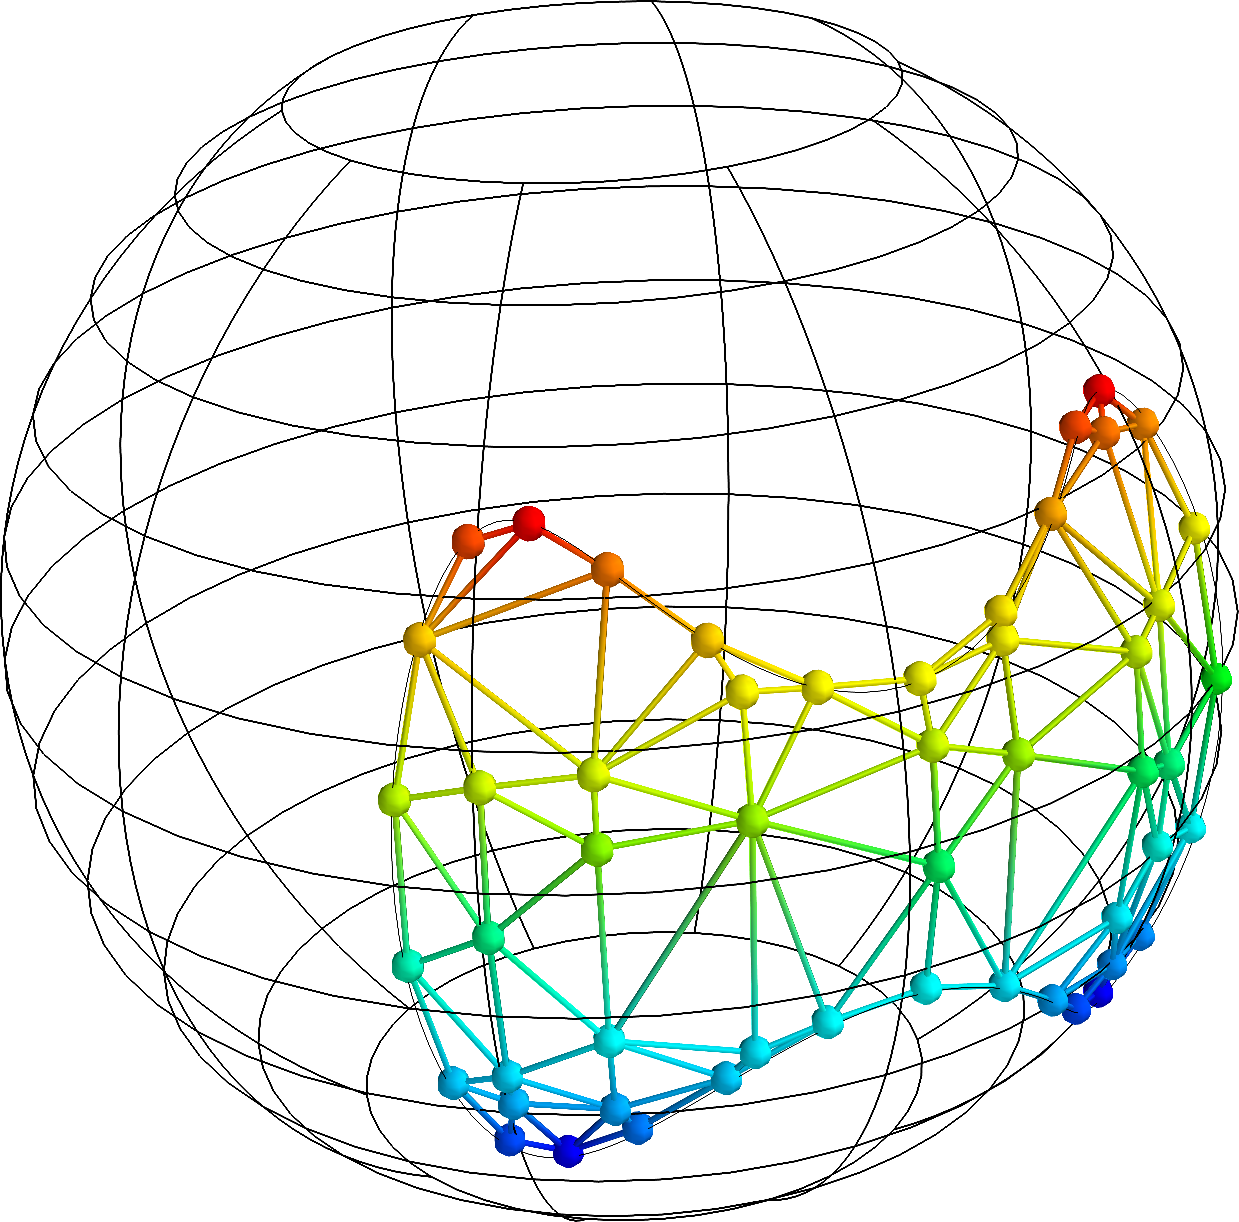
\includegraphics{manifold_simplex.png}}
\caption{Simplical decomposition for surface defined by closed curve on spherical manifold.}\label{fig5_2}
\end{center}
\end{figure} 
The only difference between the derivation of the fundamental theorem of geometical calculus on a vector space 
(which we have proved) and on a manifold is that the pseudo-scalar is not a constant but is now a function of 
position, $\f{I}{x}$, on the manifold.  If we are not on a manifold the pseudo scalars corresponding to the 
oriented volume of each simplex are proportional to one another (they are equal when normalized) so have the
same orientation.  For a manifold the orientation of $\f{I}{x}$ can change with the position vector $x$.  
In the case of figure~\ref{fig5_2} $\f{I}{x}$ is a bi-vector defined by
the tangent space (tangent plane) for each point on the sphere.

Now consider the directed volume element (in the case of figure~\ref{fig5_2} an area element) for each simplex in
figure~\ref{fig5_2} given by $\Delta X = \bfrac{1}{k!}e_{1}\W\dots\W e_{k}$ ($k=2$ for figure~\ref{fig5_2}).  As
the volume (area) of $\Delta X\rightarrow 0$, $\Delta X \propto \f{I}{x}$.

In equation~\ref{eq279} where on the l.h.s. of the equation we are integrating over the boundary of the simplex where
$f$ is a linear approximation to an arbitrary multivector function.
\be
 \oint_{\f{\partial}{x}_{\f{}{k}}}\hspace{-15pt}\f{f}{x} = \dot{f}\dot{\nabla}\cdot\f{}{\Delta X} \nonumber
\ee
consider the operator $\dot{\nabla}\cdot\f{}{\Delta X}$ where we have left the dot on the $\nabla$ to emphasize that it is not
differentiating the $\Delta X$. On a given simplex
\be
	\nabla = e^{i}\pdiff{}{\lambda^{i}}
\ee
where the $\lambda^{i}$'s are the simplical coordinates (equation~\ref{eq237}) and the $e^{i}$'s are the reciprocal vectors to the $e_{i}$'s that
define the simplex.  In the case of a manifold as the volume of $\Delta X \rightarrow 0$ the $e_{i}$'s (since the $e^{i}$'s
define the same subspace as the $e_{i}$'s) define a pseudoscalar that is proportional to $\f{I}{x}$ so that $e^{i}\pdiff{}{\lambda^{i}}$
is the projection of the geometric derivative, $\nabla$, from the embedding vector space of the manifold to the tangent space
of the manifold at point $x$.  Thus in the case of a manifold as the volume of $\Delta X \rightarrow 0$ we have 
$\partial = e^{i}\pdiff{}{\lambda^{i}}$.

Note that
\be
	\dot{\partial}\f{}{\Delta X} = \dot{\partial}\cdot\f{}{\Delta X}+\dot{\partial}\W\f{}{\Delta X}
\ee
but $\dot{\partial}\W\f{}{\Delta X} = 0$ since $\partial$ is within the subspace (tangent space) defined by $\Delta X$.  The
fundamental theorem of geometric calculus as applied to a manifold is
\be\label{eq5_127}
	\oint_{\partial V}\f{\Llin}{dS} =  \int_{V}\f{\dot{\Llin}}{\dot{\nabla}\cdot dX} = \int_{V}\f{\dot{\Llin}}{\dot{\partial}dX}
\ee
One can write $dX = \f{I}{x}\abs{dX}$ and note that $\partial$ or $\nabla$ in equation~\ref{eq5_127} do not differentiate $\f{I}{x}$.
\subsection{Divergence Theorem on Manifolds}
Let $\f{\Llin}{A} = \grade{JAI^{-1}}{}$ where $J$ is a vector field in the tangent space of the manifold and substitute into
equation~\ref{eq5_127} to get
\be\label{eq5_128}
 \oint_{\partial V}\grade{J dS I^{-1}}{} = \int_{V}\paren{\grade{\dot{J}\dot{\partial}dXI^{-1}}{}+\grade{J\dot{\partial}dX\dot{I^{-1}}}{}}.
\ee
Now reduce equation~\ref{eq5_128} by noting that $ndS = I\abs{dS}$ where $n$ is the outward normal to the surface element $dS$. We can define
an outward normal in $n$-dimensional manifold since the grade of $dS$ is $n-1$ and it defines a subspace of the tangent space of dimension $n-1$
for which a unique normal exists. This gives
\begin{align}
dS &= \bfrac{n}{n^{2}}I\abs{dS} \\
\grade{J dS I^{-1}}{} &= \bfrac{\abs{dS}}{n^{2}}\grade{JnII^{-1}}{} \nonumber \\
                      &= \bfrac{\abs{dS}}{n^{2}}\grade{Jn}{} \nonumber \\
                      &= \bfrac{J\cdot n\abs{dS}}{n^{2}} 
\end{align}
Also
\begin{align}
\dot{J}\dot{\partial}dXI^{-1} &= \dot{J}\dot{\partial}I\abs{dX}I^{-1} \nonumber \\
                              &= \dot{J}\dot{\partial}\abs{dX} \\
\grade{\dot{J}\dot{\partial}dXI^{-1}}{} &= \grade{\dot{J}\dot{\partial}\abs{dX}}{} \nonumber \\
                                        &= \grade{\dot{J}\dot{\partial}}{}\abs{dX} \nonumber \\
                                        &= \partial\cdot J\abs{dX}.
\end{align}
Finally, since both $I^{-1}$ and $dX$ are proportional to $I$
\begin{align}
\grade{J\dot{\partial}\dot{I^{-1}}dX}{} &= \pm\grade{J\dot{\partial}\dot{I}I}{}\abs{dX} \nonumber \\
                                        &= \pm\bfrac{1}{2}\grade{J\dot{\partial}\f{}{\dot{I}I+I\dot{I}}}{}\abs{dX} \nonumber \\
                                        &= \pm\bfrac{1}{2}\grade{J\partial\f{}{I^{2}}}{}\abs{dX} \nonumber \\
                                        &= 0
\end{align}
so that the divergence theorem is 
\be
 \oint_{\partial V}\bfrac{n}{n^{2}}\cdot J \abs{dS} = \int_{V}\partial\cdot J\abs{dX}
\ee
\subsection{Stokes Theorem on Manifolds}
Assume that the manifold tangent space dimension is $s+1$ and $B_{r}$ is a grade $r$ multivector field.  For clarity we denote
the grade of volume and surface elements with a subscript on the $d$'s so that $dX = d_{s+1}X$ and $dS = d_{s}S$.  Now let
$\f{\Llin}{A} = \grade{B_{r}A}{\abs{s-r}}$ so that the application of equation~\ref{eq5_127} gives
\begin{align}\label{eq5_135}
	\oint_{\partial V}\grade{B_{r}d_{s}S}{\abs{s-r}} &= \int_{V}\grade{\dot{B}_{r}{\dot{\partial}}d_{s+1}X}{\abs{s-r}} \nonumber \\
	\oint_{\partial V}\overbrace{B_{r}\cdot d_{s}S}^{\mbox{grade $\abs{s-r}$}} &= \int_{V}\grade{\f{}{\overbrace{\dot{B}_{r}\W\dot{\partial}}^{\mbox{grade $r+1$}}+
	                                       \underbrace{\dot{B}_{r}\cdot\dot{\partial}}_{\mbox{grade $r-1$}}}d_{s+1}X}{\abs{s-r}} \nonumber \\
                                            &= \paren{-1}^{r}\int_{V}\grade{\underbrace{\paren{\partial\W B_{r}}d_{s+1}X}_{\mbox{lowest grade is $\abs{s-r}$}}}{\abs{s-r}}
                                               +\int_{V}\grade{\underbrace{\paren{\dot{B}_{r}\cdot\dot{\partial}}d_{s+1}X}_{\mbox{lowest grade is $\abs{s-r+2}$}}}{\abs{s-r}} \nonumber \\
                                            &= \paren{-1}^{r}\int_{V}\paren{\partial\W B_{r}}\cdot d_{s+1}X
\end{align}
However 
\be
 	\paren{\partial\W B_{r}}\cdot d_{s+1}X = \paren{D\W B_{r}}\cdot d_{s+1}X  
\ee
since $d_{s+1}X = \f{I_{s+1}}{x}\abs{d_{s+1}X}$ and the dot product of any component of $\partial\W B_{r}$ that is not in the tangent space defined by $\f{I_{s+1}}{x}$ is zero so that
\be\label{eq5_137}
	\oint_{\partial V}B_{r}\cdot d_{s}S = \int_{V}\paren{\dot{B}_{r}\W\dot{D}}\cdot d_{s+1}X = \paren{-1}^{r}\int_{V}\paren{D\W B_{r}}\cdot d_{s+1}X
\ee
The divergence theorem is recovered when $r=s-1$.  This is important for constructing conservation theorems in curved spaces. Equation~\ref{eq5_137} is the most
general application of equation~\ref{eq5_127} that allows one to replace $\partial$ with $D$ (covariant derivative) on a manifold.
